\documentclass[10pt,twocolumn,letterpaper]{article}
\usepackage[margin=0.75in]{geometry}
\usepackage{times}
\usepackage{helvet}
\usepackage{courier}
\usepackage[hyphens]{url}
\usepackage{graphicx}
\usepackage{booktabs}
\usepackage{multirow}
\usepackage{amsmath}
\usepackage{float}
\urlstyle{rm}
\usepackage{natbib}
\usepackage{caption}
\frenchspacing

\title{\LARGE \bf TeleMed-M3: Dynamic Imputation-Free Multimodal Learning for Explainable Metabolic Disease Risk Stratification}
\author{
    Gunda Swaran\textsuperscript{1}, Kolipaka Vishal\textsuperscript{1}, Pagidipalli Sunny Kiran\textsuperscript{1}, \\
    Chikyala Medhansh Rao\textsuperscript{1}, Aitha Thadhagath Ram\textsuperscript{1} \\
    \\
    \textsuperscript{1}Keshav Memorial Institute of Technology, Hyderabad, India \\
    {\tt\small \{swarangunda23, kolipakavishal06, sunnykmithyd,}\\ \vspace{2pt} {\tt\small medhanshrao.07, thadhagath.ram.aitha1108\}@gmail.com}
}
\date{}

\begin{document}
\maketitle

\begin{abstract}
Cardiometabolic conditions---Type~2 Diabetes (T2D), Prediabetes, High Adiposity Risk, Metabolic Syndrome, and Non-Alcoholic Fatty Liver Disease (NAFLD)---arise from intricate interactions among laboratory biomarkers, lifestyle patterns, and microbial ecology. Present-day telehealth platforms predominantly leverage clinical records and wearable telemetry, yet seldom incorporate gut microbiome profiles or offer principled strategies for handling absent data channels. We introduce TeleMed-M3, a modular multimodal predictive framework embedded within a Generative-AI-assisted telemedicine system for individualized metabolic risk assessment. The architecture trains fifteen modality-specific expert classifiers---one per combination of three input channels (Clinical, Wearable/CGM, Gut Microbiome) and five disease targets---then fuses their calibrated probability outputs through an L2-regularized logistic regression meta-learner trained on five-fold stratified out-of-fold predictions. A deterministic routing layer directs each patient through one of seven non-empty modality-availability pathways ($2^{3}-1$ subsets), thereby circumventing the need to synthetically reconstruct any wholly absent modality block. TreeSHAP furnishes per-prediction feature attributions for the tree-based experts, and an exploratory Medical Retrieval-Augmented Generation module grounds risk summaries in retrieved clinical guidelines. Experiments on a 100{,}000-record synthetic cohort spanning 82 features reveal that the complete Clinical+Wearable+Gut pathway attains AUROCs of 0.7834 (T2D), 0.7586 (Metabolic Syndrome), and 0.7772 (NAFLD), while the routing mechanism sustains an AUROC of 0.7743 for T2D under 30\% modality-level missingness---exceeding a median-imputation baseline by 0.0021. Comparisons with early feature-level fusion confirm that probability-level routing achieves comparable or superior discrimination across all targets, with a notable advantage for Prediabetes (0.5875 vs.\ 0.5470). All findings derive from synthetic data; clinical validation on human cohorts remains a prerequisite for deployment.
\end{abstract}

\textbf{Keywords:} Multimodal Machine Learning, Gut Microbiome, Telemedicine, Dynamic Modality Routing, Explainable AI, TreeSHAP, Retrieval-Augmented Generation, Metabolic Disease Risk Stratification

\section{INTRODUCTION}

\subsection{Background}
Metabolic disorders constitute a rapidly expanding global health burden. T2D alone affects hundreds of millions of individuals worldwide, and closely related conditions---Prediabetes, elevated adiposity, Metabolic Syndrome, and NAFLD---frequently co-occur, amplifying cardiovascular and hepatic morbidity \citep{topol2019high}. Accurate risk stratification therefore demands a holistic view of patient physiology that spans multiple measurement domains.

Three complementary data streams are particularly informative. First, standard clinical assessments---encompassing anthropometrics, fasting glucose, glycated hemoglobin, lipid panels, and hepatic enzymes---capture snapshot physiology during clinic visits \citep{rajkomar2018scalable}. Second, wearable sensors and Continuous Glucose Monitoring (CGM) devices record longitudinal behavioral and glycemic patterns that periodic laboratory tests cannot capture \citep{hall2018glucotypes}. Third, metagenomic profiling of the gut microbiome quantifies microbial taxa and ecological indices implicated in insulin resistance, systemic inflammation, and energy harvest \citep{qin2012metagenome, turnbaugh2006obesity}.

Despite the recognized value of each source, practical telehealth systems rarely unify all three within a single analytic pipeline. Moreover, real-world patient encounters frequently present incomplete modality coverage: a patient may possess laboratory results and wearable logs but lack a recent stool sequencing report, or may have microbiome data without contemporaneous CGM readings. Conventional multimodal architectures that concatenate all features into a monolithic input vector are ill-suited to this scenario, as they require either discarding the patient or fabricating the missing channel through numerical imputation \citep{rubin1976inference, ma2021smil}.

\subsection{Problem Statement}
Four interrelated obstacles hinder the construction of robust multimodal metabolic risk systems within telehealth environments:

\begin{enumerate}
    \item \textbf{Data heterogeneity.} Clinical variables, wearable time-series summaries, and high-dimensional microbiome abundance vectors differ in scale, sparsity, and acquisition cadence, complicating joint modeling.
    \item \textbf{Structural modality absence.} Entire measurement channels may be unavailable for individual patients---not merely individual features---rendering standard feature-level imputation conceptually inappropriate.
    \item \textbf{Opacity of predictions.} Ensemble and gradient-boosted classifiers common in tabular health analytics often function as opaque decision systems, limiting clinician trust and actionability.
    \item \textbf{Evidence grounding.} Raw probability scores lack clinical context; translating them into guideline-referenced narratives requires coupling predictive models with curated medical knowledge.
\end{enumerate}

An effective framework must therefore accommodate variable modality availability at inference time, supply transparent per-feature explanations, and optionally situate its outputs within established clinical evidence.

\subsection{Research Gap}
Prior work has advanced healthcare prediction from electronic health records \citep{rajkomar2018scalable, esteva2019guide}, explored wearable-derived biomarkers for glycemic phenotyping \citep{zeevi2015personalized, hall2018glucotypes}, characterized gut microbial signatures of metabolic dysfunction \citep{qin2012metagenome, turnbaugh2006obesity}, and developed general multimodal fusion strategies \citep{huang2020multimodal}. Missing-modality techniques based on reconstruction, dropout regularization, or latent-space alignment have also been proposed \citep{ma2021smil}. However, these threads are typically pursued in isolation or under architectures that presume a fixed set of input modalities.

An integrated framework that (i) trains dedicated per-modality experts across clinical, wearable, and microbiome channels, (ii) fuses their outputs at the probability level through stacking, (iii) dynamically selects among all non-empty modality subsets without imputing absent blocks, (iv) furnishes game-theoretic feature attributions, and (v) incorporates retrieval-augmented report generation---has not been systematically investigated for multi-target metabolic risk stratification.

\subsection{Research Questions}
\begin{itemize}
    \item \textbf{RQ1:} What discriminative performance do the standalone Clinical, Wearable/CGM, and Gut Microbiome experts achieve for each of the five metabolic risk targets?
    \item \textbf{RQ2:} How does late probability-level stacking across the seven modality-availability pathways compare to single-modality baselines?
    \item \textbf{RQ3:} Does incorporating additional modalities yield measurable gains beyond Clinical-only prediction?
    \item \textbf{RQ4:} How resilient is the dynamic routing mechanism when entire modality blocks are randomly withheld at inference?
    \item \textbf{RQ5:} Does routing outperform conventional median imputation of absent modality blocks?
    \item \textbf{RQ6:} How does the proposed probability-level routing compare with a standard early feature-concatenation baseline?
    \item \textbf{RQ7:} Can TreeSHAP explanations and retrieval-augmented generation be meaningfully integrated to support clinician-oriented risk communication?
\end{itemize}

\subsection{Contributions}
The principal contributions of this work are:
\begin{itemize}
    \item \textbf{Unified Trimodal Telehealth Architecture.} A modular pipeline that ingests Clinical, Wearable/CGM, and Gut Microbiome measurements and delivers calibrated risk scores for five metabolic conditions within a single telemedicine environment.
    \item \textbf{Imputation-Free Seven-Pathway Routing.} A deterministic routing layer enumerating all $2^{3}-1$ non-empty modality subsets, enabling inference under arbitrary patterns of modality absence without synthetic reconstruction of unobserved data.
    \item \textbf{Out-of-Fold Probability Stacking.} A meta-learner trained on five-fold stratified out-of-fold expert predictions, mitigating information leakage between the base and fusion stages.
    \item \textbf{Interpretable Risk Attribution.} Integration of TreeSHAP to decompose individual predictions from tree-based experts into per-feature contribution scores.
    \item \textbf{Evidence-Grounded Generative Reporting.} An exploratory Medical RAG module that retrieves relevant clinical guidelines and synthesizes them with structured model outputs to produce human-readable health summaries.
    \item \textbf{Comprehensive Synthetic Benchmark.} Systematic evaluation across seven pathways, three missingness rates, a median-imputation baseline, and an early-fusion comparator on a 100{,}000-patient controlled cohort.
\end{itemize}

\section{RELATED WORK}

\subsection{Machine Learning for Electronic Health Records}
The application of supervised learning to structured clinical data has demonstrated substantial promise for patient phenotyping, readmission prediction, and mortality forecasting \citep{rajkomar2018scalable}. Deep architectures and gradient-boosted ensembles such as XGBoost \citep{chen2016xgboost} and LightGBM \citep{ke2017lightgbm} have achieved competitive discrimination on tabular health datasets. Nonetheless, models trained exclusively on point-in-time laboratory values may overlook behavioral and biological dynamics captured by complementary measurement modalities \citep{topol2019high}.

\subsection{Wearable Sensors and Continuous Glucose Monitoring}
Ambulatory devices that record heart rate, activity counts, sleep architecture, and interstitial glucose concentration offer a longitudinal physiological perspective unavailable from periodic clinic visits \citep{hall2018glucotypes}. Zeevi et al.\ demonstrated that integrating CGM traces with clinical and microbiome features substantially improved postprandial glycemic response prediction \citep{zeevi2015personalized}. These findings underscore the potential of wearable telemetry as a complementary input channel, while also highlighting challenges of variable device adherence and signal quality across patient populations.

\subsection{Gut Microbiome and Metabolic Pathophysiology}
Metagenome-wide association studies have linked compositional shifts in intestinal microbial communities---particularly reduced Bacteroidetes-to-Firmicutes ratios and diminished butyrate-producing taxa---to insulin resistance, obesity, and hepatic steatosis \citep{qin2012metagenome, turnbaugh2006obesity}. Ecological diversity indices and functional pathway abundances can serve as predictive features for metabolic disease classifiers. However, microbiome profiling remains costly and is infrequently available in routine telehealth encounters, motivating architectures that can gracefully operate in its absence.

\subsection{Multimodal Fusion Strategies}
Multimodal learning seeks to exploit the complementarity among heterogeneous data sources \citep{huang2020multimodal}. Fusion can occur at the feature level (early concatenation), the representation level (intermediate shared embeddings), or the decision level (late combination of per-modality predictions). While feature-level fusion is straightforward, it couples the model to a rigid input schema and is sensitive to dimensionality imbalance. Probability-level stacking, originally formalized as stacked generalization \citep{wolpert1992stacked}, decouples modality-specific learning from cross-modal combination and naturally accommodates variable-width input vectors.

\subsection{Handling Missing Modalities}
Absent data channels pose a distinct challenge from missing individual features. Standard imputation methods---mean/median filling, iterative chained equations, or $k$-nearest-neighbor interpolation---address sporadic feature-level gaps \citep{rubin1976inference}. When an entire modality is unavailable, reconstruction-based methods attempt to hallucinate the absent representation via generative models or cross-modal translation \citep{ma2021smil}. An alternative philosophy is to avoid fabrication altogether by routing patients through pathway-specific fusion models conditioned only on observed modalities. TeleMed-M3 adopts this routing approach, training separate meta-learners for every non-empty modality subset.

\subsection{Explainability and Retrieval-Augmented Generation}
SHAP values, grounded in cooperative game theory, decompose each prediction into additive per-feature contributions \citep{lundberg2017unified}. The TreeSHAP variant achieves exact Shapley computation in polynomial time for tree-ensemble models, making it well suited to the gradient-boosted experts employed in this work. Separately, Retrieval-Augmented Generation (RAG) conditions language-model outputs on passages retrieved from an external corpus, reducing hallucination and anchoring generated text in verifiable sources \citep{lewis2020retrieval}. Combining TreeSHAP attributions with RAG-retrieved clinical guidelines offers a pathway toward risk reports that are simultaneously data-driven and evidence-grounded \citep{esteva2019guide}.

\section{DATASET AND COHORT}

\subsection{Synthetic Cohort Construction}
Privacy regulations and the scarcity of publicly available datasets containing synchronized clinical, wearable, and microbiome measurements for identical individuals necessitated the creation of a synthetic evaluation cohort. A Gaussian Copula latent variable model \citep{xu2015sdv} was employed to generate 100{,}000 patient records whose inter-feature correlations replicate established physiological relationships---for instance, the covariance between insulin resistance markers and inflammatory cytokines, or between gut dysbiosis indices and hepatic enzyme elevations. Stochastic binomial sampling translated continuous disease liability scores into binary ground-truth labels for each target.

\subsection{De-Clamping and Leakage Prevention}
The generative process deliberately avoided deterministic clamping rules that would permit classifiers to reverse-engineer the data-generation logic. Instead, probabilistic biological variance and additive noise were injected into all feature--target relationships, ensuring that predictive performance reflects learned statistical associations rather than memorized generation artifacts. Rigorous data-isolation protocols prevented any cross-modality meta-level target leakage during synthesis.

\subsection{Feature and Modality Composition}
The resulting dataset encompasses 82 predictive features partitioned across three modality blocks:
\begin{itemize}
    \item \textbf{Clinical (18 features):} Anthropometric measures (Age, BMI, Waist Circumference) and laboratory biomarkers (Fasting Glucose, HbA1c, Triglycerides, LDL/HDL Cholesterol, ALT, AST, GGT, among others).
    \item \textbf{Wearable/CGM (15 features):} Continuous physiological telemetry comprising mean and resting heart rate, heart rate variability, daily step count, active minutes, sleep duration, sleep efficiency, and glucose variability statistics derived from CGM traces.
    \item \textbf{Gut Microbiome (49 features):} Relative abundances of 40 bacterial taxa (e.g., Firmicutes, Bacteroidetes, \textit{Akkermansia muciniphila}, \textit{Faecalibacterium prausnitzii}) together with 9 ecological and functional indices including Shannon Diversity, Chao1 Richness, and short-chain fatty acid pathway scores.
\end{itemize}

\subsection{Prediction Targets}
Five binary classification targets, each representing a distinct yet pathophysiologically interconnected metabolic condition, are independently evaluated:
\begin{enumerate}
    \item Type~2 Diabetes (T2D)
    \item Prediabetes
    \item High Adiposity Risk
    \item Metabolic Syndrome
    \item Non-Alcoholic Fatty Liver Disease (NAFLD)
\end{enumerate}
Prediabetes and T2D were constrained to be mutually exclusive within the generative model, reflecting standard diagnostic boundaries.

\subsection{Cohort Prevalence}
The prevalence rates in the 100{,}000-patient cohort are: T2D 52.6\%, Prediabetes 20.0\%, High Adiposity Risk 39.0\%, Metabolic Syndrome 57.1\%, and NAFLD 59.6\%. These rates were calibrated to approximate epidemiological distributions while maintaining sufficient positive-class representation for stable classifier training.

\subsection{Data Partitioning}
A deterministic 70/15/15 split yielded three non-overlapping partitions:
\begin{itemize}
    \item \textbf{Training (70{,}000 patients):} Used for fitting the 15 modality-specific experts and for generating out-of-fold predictions to train the meta-learner.
    \item \textbf{Validation (15{,}000 patients):} Reserved for hyperparameter selection and early-stopping criteria.
    \item \textbf{Test (15{,}000 patients):} Strictly held out for all reported performance metrics and missingness simulations.
\end{itemize}

\section{METHODOLOGY}

\begin{figure*}[t]
\centering
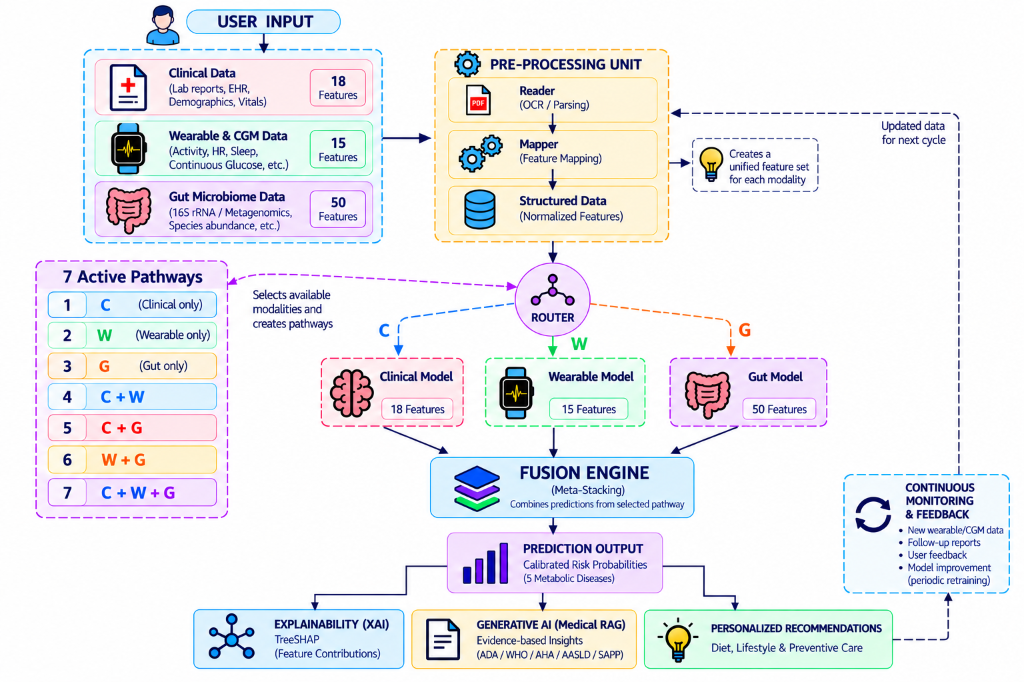
\includegraphics[width=\textwidth]{figures/architecture.png}
\caption{System architecture of TeleMed-M3. Patient data is partitioned into Clinical (18 features), Wearable/CGM (15 features), and Gut Microbiome (49 features) blocks. Modality-specific experts produce per-target risk probabilities, which a dynamic router channels through one of seven pathways to an L2-regularized meta-learner. TreeSHAP attributions and Medical RAG summaries are generated downstream.}
\label{fig:arch}
\end{figure*}

\subsection{Architectural Overview}
Figure~\ref{fig:arch} depicts the end-to-end pipeline of TeleMed-M3. Upon ingestion, each patient record is segmented into its constituent modality blocks. Independent expert classifiers process each block to emit per-target risk probabilities. A deterministic routing layer inspects which modality blocks are present and dispatches the corresponding probability vector to the appropriate pathway-specific meta-learner. Post-fusion, TreeSHAP generates local feature attributions for supported tree-based experts, and an optional Medical RAG module synthesizes the structured outputs into evidence-grounded narrative summaries.

\subsection{Modality-Specific Expert Models}
Fifteen expert classifiers are trained---one for each pairing of three modalities and five disease targets. For every modality--target combination, the best-performing algorithm was selected from a candidate pool comprising Logistic Regression, XGBoost \citep{chen2016xgboost}, LightGBM \citep{ke2017lightgbm}, CatBoost, and ExtraTrees. Consequently, the expert ensemble is heterogeneous: different modality--target slots may be served by different classifier families, reflecting the varying predictive structure of each subproblem.

Each expert incorporates an internal preprocessing stage that handles feature-level missing values within its modality block---for example, median filling of sporadic NaN entries---using transformations appropriate to the selected estimator. This intra-modality imputation is conceptually distinct from the inter-modality routing mechanism, which addresses the wholesale absence of an entire data channel.

\subsection{Out-of-Fold Probability Generation and Stacking}
To prevent information leakage between the expert and fusion stages, meta-learner training features are constructed through five-fold stratified cross-validation over the 70{,}000-patient training partition. In each fold, an expert model fitted on four folds produces predicted probabilities for the held-out fifth fold. Concatenating these out-of-fold (OOF) probabilities across all five folds yields a complete set of uncontaminated meta-features \citep{wolpert1992stacked}.

An L2-regularized Logistic Regression meta-learner then learns to optimally combine the expert probabilities for each target. This probability-level stacking preserves the calibration properties of each expert's output and avoids the curse of dimensionality that arises when concatenating 82 raw features directly.

\subsection{Seven-Pathway Dynamic Routing}
Three binary modality-availability indicators generate $2^{3}-1=7$ non-empty subsets: C, W, G, C+W, C+G, W+G, and C+W+G. For each subset and each target, a dedicated meta-learner is trained on the corresponding column subset of the OOF probability matrix.

At inference, the router examines which modality blocks are present for a given patient and forwards only the corresponding expert probabilities to the matching pathway meta-learner. If a modality is entirely absent, its expert is never invoked and no synthetic probability is fabricated. This structural routing approach contrasts with imputation-based alternatives, which would fill the absent block with estimated values and feed them through a single fixed-input model.

\subsection{TreeSHAP Explainability}
For each tree-based expert, TreeSHAP \citep{lundberg2017unified} computes exact Shapley values in time polynomial in the number of leaves, decomposing each prediction into signed per-feature contributions. These attributions identify which clinical biomarkers, wearable signals, or microbial taxa most influenced the risk score for an individual patient. The explanations are intended as interpretive aids for healthcare professionals and do not imply causal relationships.

\subsection{Medical Retrieval-Augmented Generation}
An exploratory Medical RAG module augments the structured model outputs with contextual clinical knowledge. A FAISS-indexed corpus of medical guidelines---drawing on resources such as ADA Standards of Care and AHA cardiovascular risk recommendations---supplies relevant passages at inference time. A large language model then synthesizes the retrieved evidence, TreeSHAP attributions, and predicted probabilities into a coherent, patient- or clinician-facing narrative. This component is positioned as a proof-of-concept reporting layer; its retrieval precision, generation fidelity, and hallucination rate were not quantitatively benchmarked in the current study.

\section{EXPERIMENTAL DESIGN}

\subsection{Evaluation Metrics}
All reported results are computed on the sequestered 15{,}000-patient test partition. Four complementary metrics characterize predictive quality:
\begin{itemize}
    \item \textbf{AUROC:} Measures rank-order discrimination irrespective of threshold selection.
    \item \textbf{AUPRC:} Quantifies precision--recall trade-offs, informative under class imbalance.
    \item \textbf{F1-Score:} Harmonic mean of precision and recall at a fixed decision threshold of 0.5, with no post-hoc threshold tuning on the test set.
    \item \textbf{Brier Score:} Assesses the mean squared deviation between predicted probabilities and observed binary outcomes, capturing both calibration and discrimination \citep{brier1950verification}.
\end{itemize}

\subsection{Simulated Modality-Level Missingness}
To probe the robustness of dynamic routing under incomplete data availability, entire modality blocks were randomly withheld from test-set patients at rates of 10\%, 20\%, and 30\%. Modality removal was applied independently and uniformly across patients, operationalizing a Missing Completely At Random (MCAR) assumption. The router then selected the appropriate pathway for each patient based on whichever modality blocks remained available.

This controlled simulation does not capture informative missingness patterns---Missing At Random (MAR) or Missing Not At Random (MNAR)---that may arise in clinical practice.

\subsection{Baseline Comparators}
Two reference strategies provide context for the proposed routing mechanism:

\textbf{Median-Imputation Baseline.} When a modality block is entirely absent, its features are replaced with the global training-set median values prior to expert prediction. The full C+W+G meta-learner then consumes all three expert outputs, including those generated from imputed inputs. This approach tests whether numerically reconstructing an absent channel yields better or worse discrimination than omitting it entirely.

\textbf{Early-Fusion Baseline.} All 82 features from the three modalities are concatenated into a single input vector, and a unified classifier is trained on the combined representation. This standard feature-level fusion strategy serves as a point of comparison for the probability-level stacking architecture. Advanced imputation techniques such as MICE or deep generative completion were not evaluated.

\section{RESULTS}

\subsection{Discrimination Across Seven Pathways}
Table~\ref{tab:fusion} presents the AUROC achieved by each of the seven modality-availability pathways for all five disease targets, addressing RQ1 through RQ3.

\begin{table*}[t]
\centering
\caption{AUROC across the seven modality-availability pathways. Single columns (C, W, G) reflect individual expert performance; compound columns reflect late probability-level fusion.}
\label{tab:fusion}
\begin{tabular}{@{}l ccccccc@{}}
\toprule
\textbf{Target} & \textbf{C} & \textbf{W} & \textbf{G} & \textbf{C+W} & \textbf{C+G} & \textbf{W+G} & \textbf{C+W+G} \\
\midrule
Type2\_Diabetes & 0.7777 & 0.6772 & 0.5949 & 0.7825 & 0.7788 & 0.6894 & 0.7834 \\
Prediabetes & 0.5839 & 0.5429 & 0.5134 & 0.5875 & 0.5840 & 0.5428 & 0.5875 \\
High\_Adiposity\_Risk & 0.7532 & 0.6602 & 0.5263 & 0.7547 & 0.7532 & 0.6607 & 0.7547 \\
Metabolic\_Syndrome & 0.7581 & 0.6207 & 0.5777 & 0.7586 & 0.7581 & 0.6336 & 0.7586 \\
NAFLD & 0.7743 & 0.5995 & 0.6487 & 0.7745 & 0.7771 & 0.6621 & 0.7772 \\
\bottomrule
\end{tabular}
\end{table*}

Across all targets, the Clinical expert consistently delivered the highest standalone discrimination, followed by the Wearable expert and then the Gut expert. For T2D, Clinical alone achieved an AUROC of 0.7777, while the complete three-modality pathway reached 0.7834---a net gain of 0.0057. Analogous modest improvements were observed for the remaining targets. Notably, the Wearable+Gut pathway, which operates without any clinical input, sustained a T2D AUROC of 0.6894, demonstrating that the non-clinical channels retain meaningful predictive signal when laboratory data is unavailable.

\begin{figure}[t]
\centering
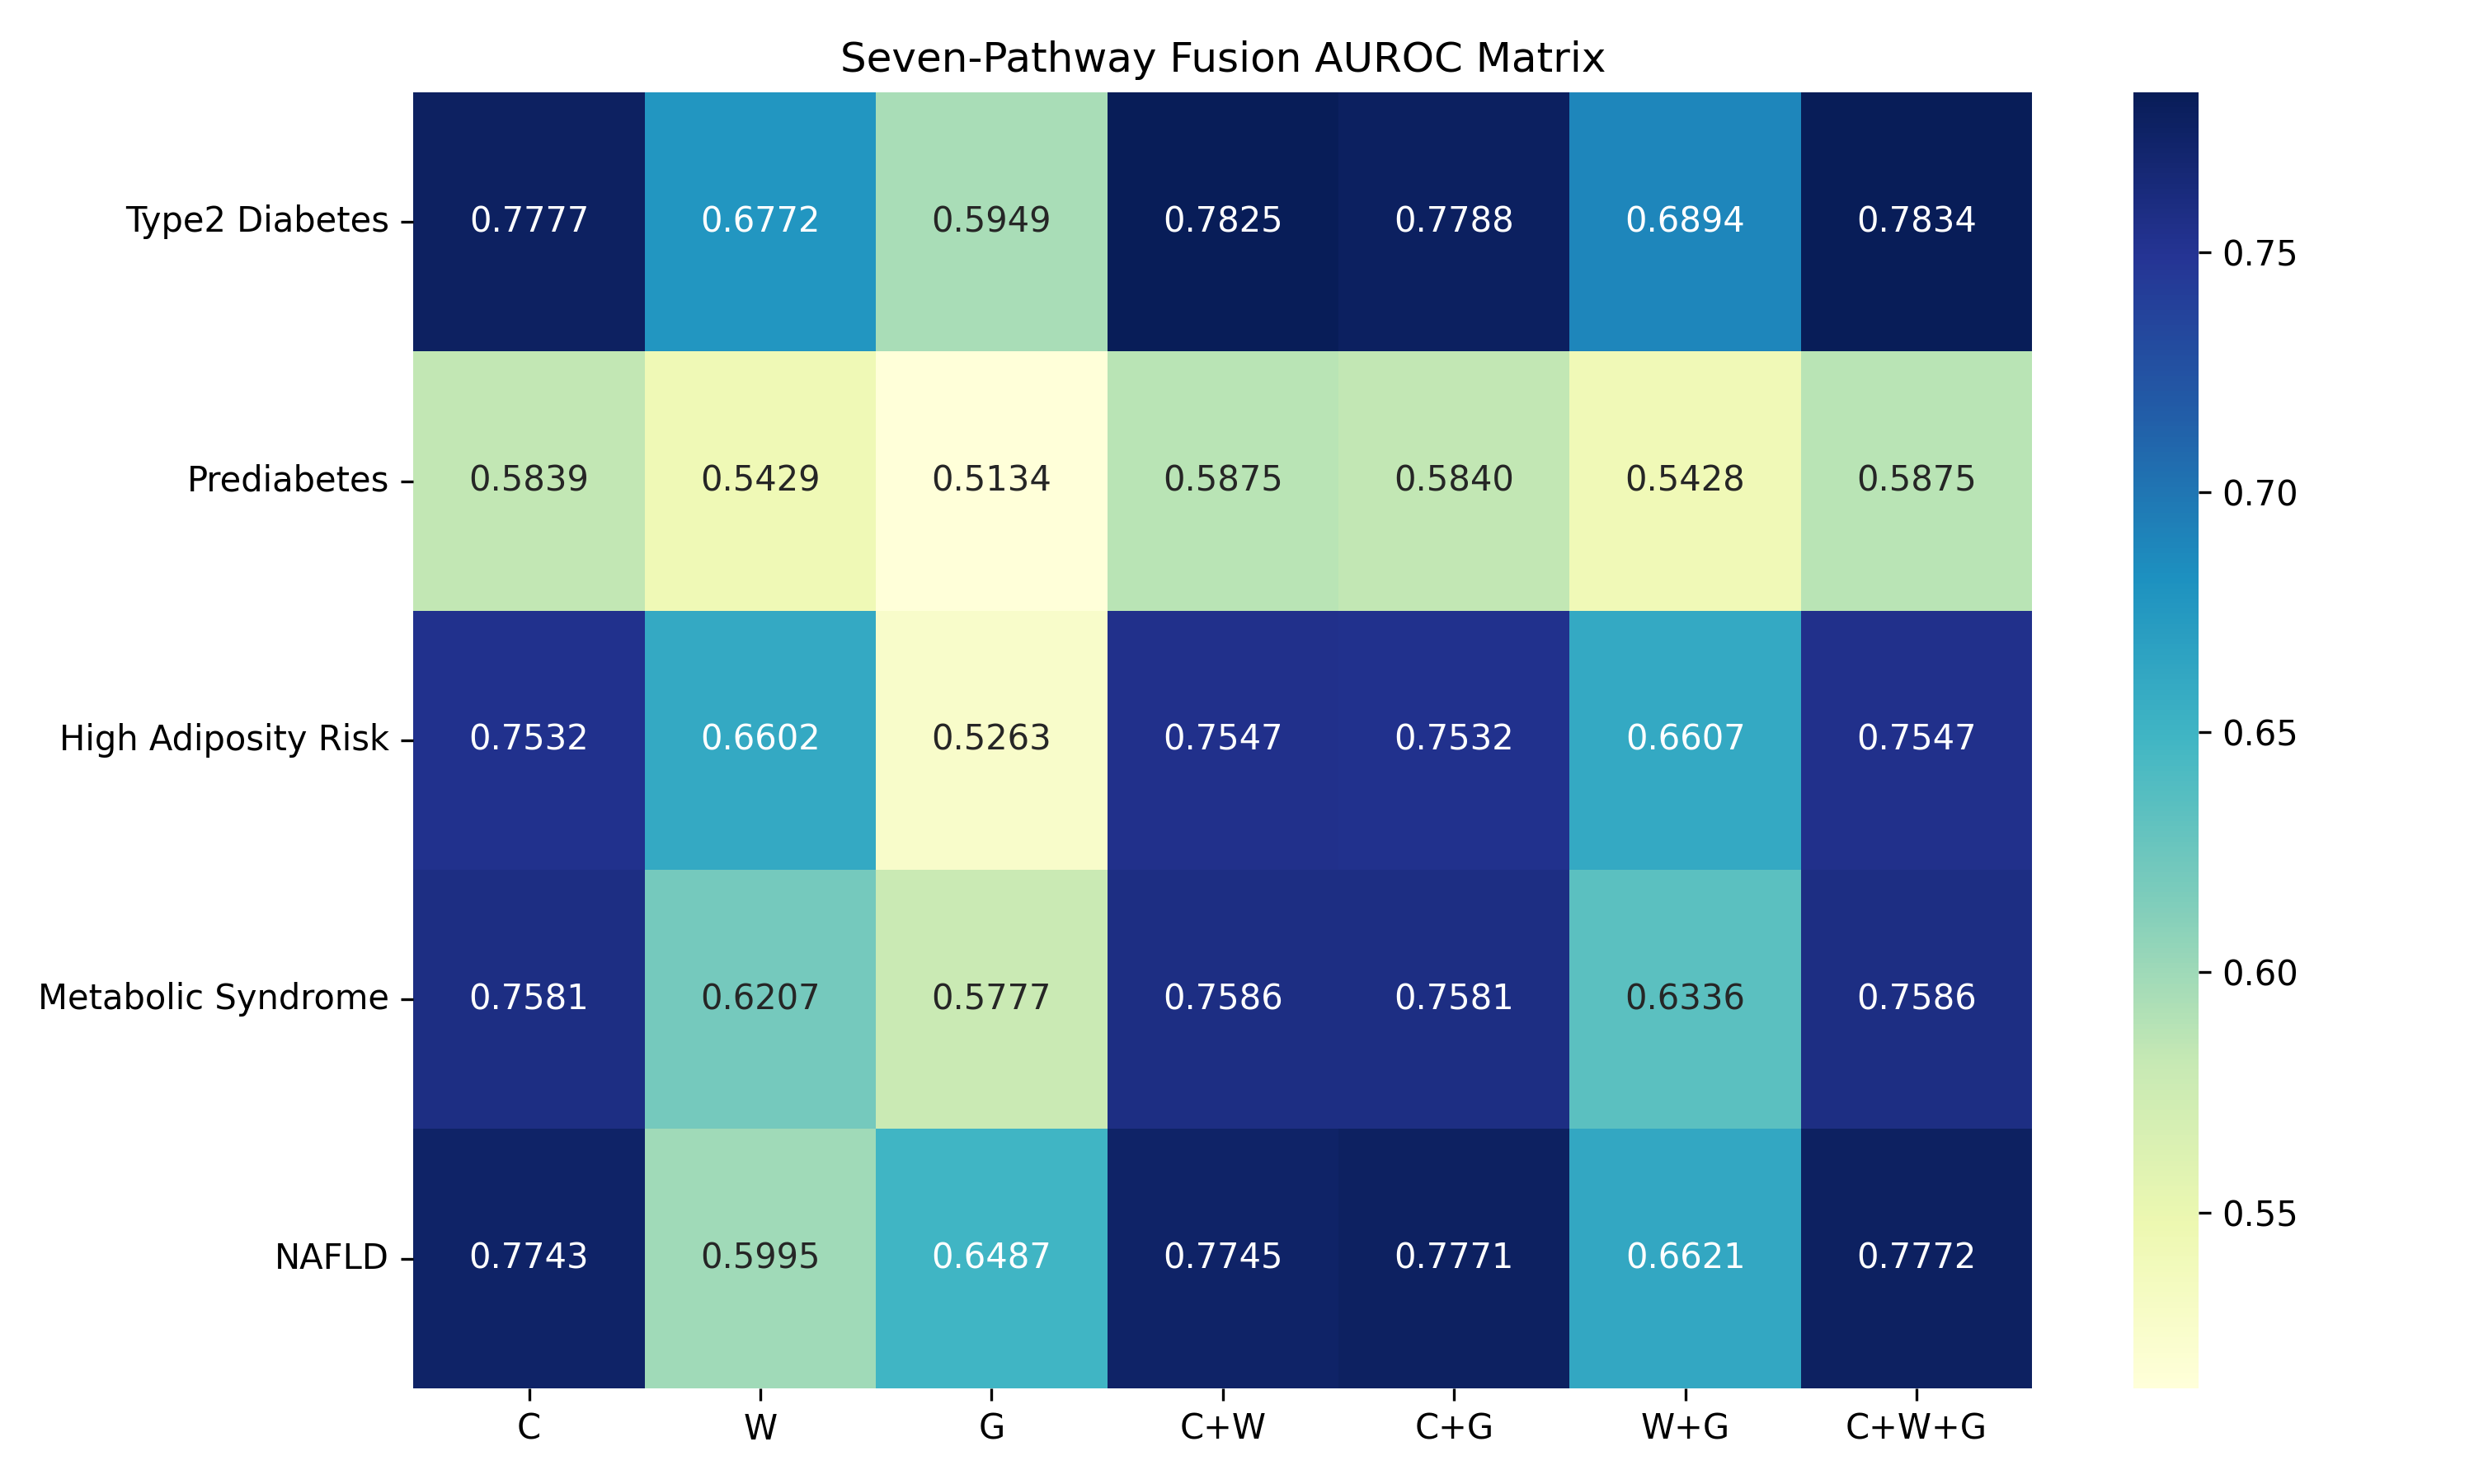
\includegraphics[width=\columnwidth]{figures/fig_pathway_auroc_heatmap.png}
\caption{Heatmap of AUROC values across the seven modality-availability pathways and five metabolic disease targets.}
\end{figure}

\subsection{Full Classification Metrics for C+W+G}
Table~\ref{tab:metrics} reports AUPRC, F1, and Brier Score for the complete trimodal pathway.

\begin{table}[t]
\centering
\caption{Extended classification metrics for the C+W+G pathway on the held-out test set.}
\label{tab:metrics}
\begin{tabular}{@{}l ccc@{}}
\toprule
\textbf{Target} & \textbf{AUPRC} & \textbf{F1} & \textbf{Brier} \\
\midrule
Type2\_Diabetes & 0.7880 & 0.7479 & 0.1898 \\
Prediabetes & 0.2431 & 0.3584 & 0.2450 \\
High\_Adiposity\_Risk & 0.6404 & 0.6475 & 0.2021 \\
Metabolic\_Syndrome & 0.7942 & 0.7600 & 0.2000 \\
NAFLD & 0.8239 & 0.7877 & 0.1927 \\
\bottomrule
\end{tabular}
\end{table}

NAFLD obtained the strongest AUPRC (0.8239) and F1 (0.7877), consistent with its relatively high prevalence and the strong hepatic biomarker signals in the clinical block. Prediabetes proved the most challenging target, with an AUPRC of only 0.2431 and an F1 of 0.3584, reflecting its low prevalence (20.0\%) and the subtlety of pre-diabetic physiological signatures in the synthetic cohort. Brier Scores ranged from 0.1898 to 0.2450, indicating moderate probabilistic calibration across targets.

\subsection{Robustness Under Simulated Missingness}
Addressing RQ4 and RQ5, Figure~\ref{fig:miss} illustrates the behavior of dynamic routing versus median imputation as the fraction of patients with missing modality blocks increases from 10\% to 30\% under MCAR conditions.

\begin{figure}[t]
\centering
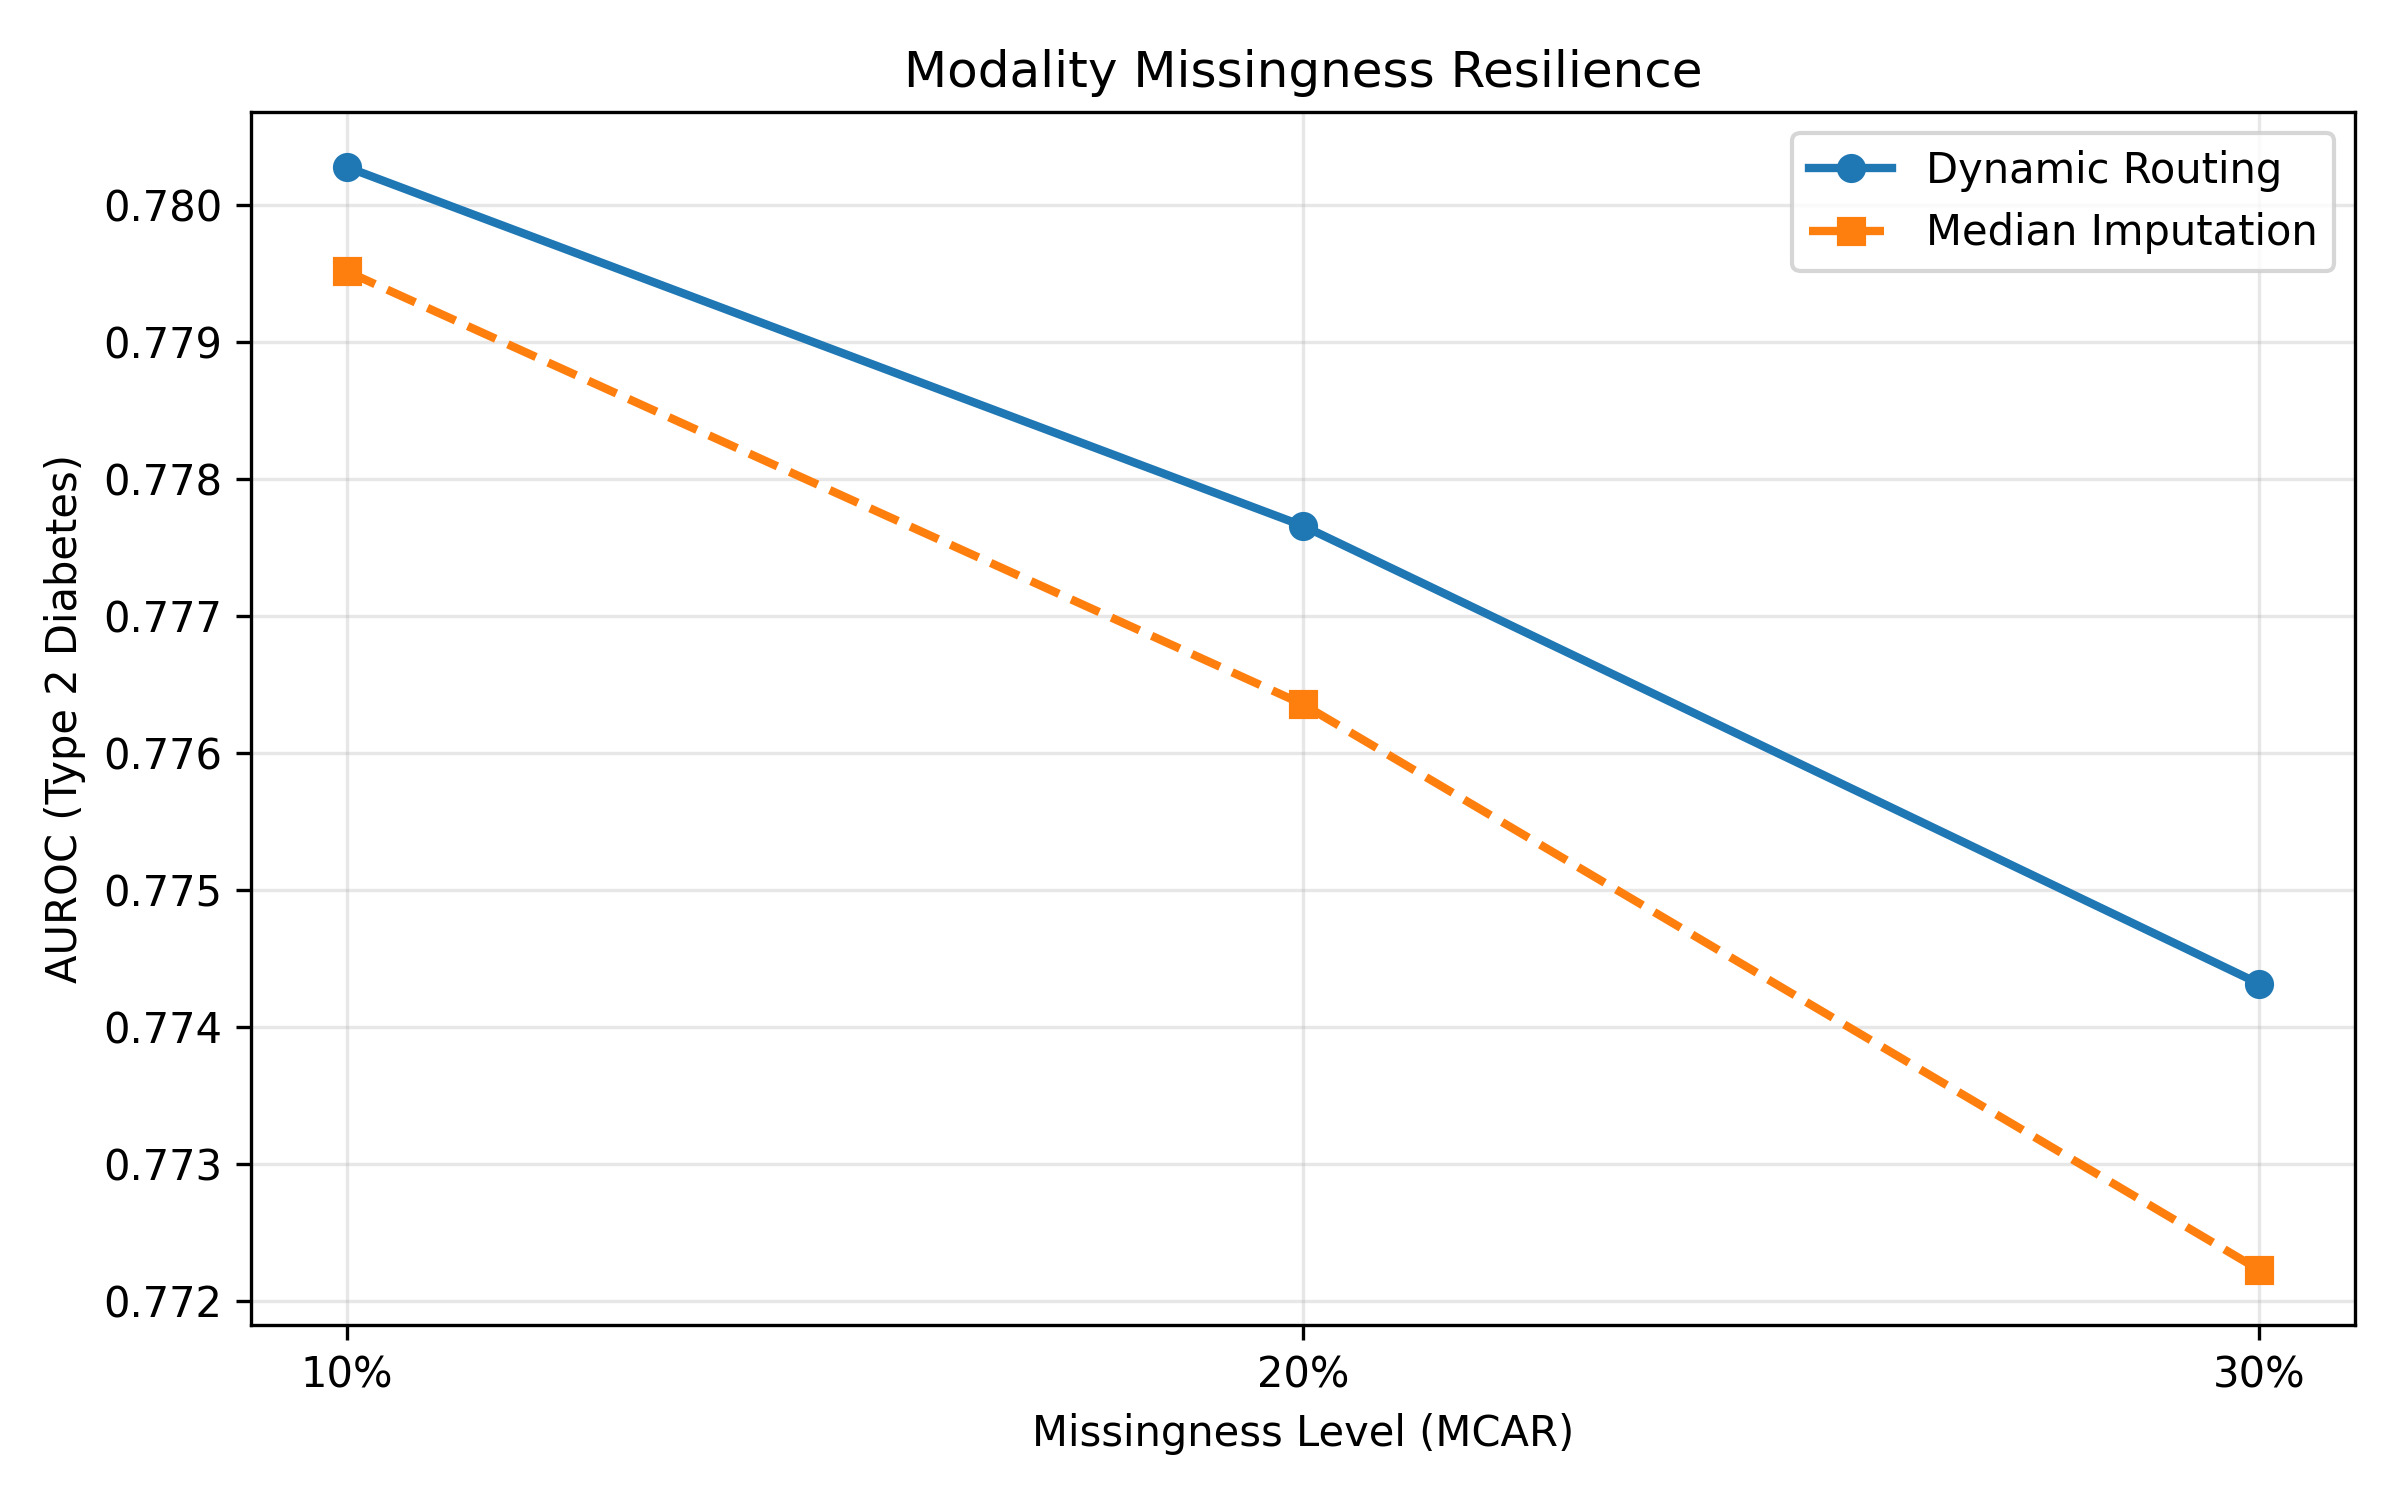
\includegraphics[width=\columnwidth]{figures/fig_missingness.png}
\caption{T2D AUROC for dynamic routing versus median imputation under 10\%, 20\%, and 30\% simulated MCAR modality-level missingness.}
\label{fig:miss}
\end{figure}

At the most severe 30\% missingness rate, dynamic routing achieved a T2D AUROC of 0.7743, compared with 0.7722 for the median-imputation strategy---a difference of 0.0021. This gap widened monotonically from 0.0007 at 10\% missingness through 0.0013 at 20\%. While the absolute magnitudes are small, the consistent direction indicates that routing patients through pathway-specific models conditioned on observed data avoids the noise introduced by populating absent modality blocks with population-level medians.

\subsection{Comparison with Early Feature-Level Fusion}
Table~\ref{tab:early} contrasts the early-fusion baseline---a single classifier operating on the concatenated 82-feature vector---with the proposed late probability-level routing (RQ6).

\begin{table}[t]
\centering
\caption{AUROC comparison between early feature-level fusion and dynamic probability-level routing.}
\label{tab:early}
\begin{tabular}{@{}l ll@{}}
\toprule
\textbf{Target} & \textbf{Early Fusion} & \textbf{Dynamic} \\
\midrule
Type2\_Diabetes & 0.7836 & 0.7834 \\
Prediabetes & 0.5470 & 0.5875 \\
High\_Adiposity\_Risk & 0.7557 & 0.7547 \\
Metabolic\_Syndrome & 0.7591 & 0.7586 \\
NAFLD & 0.7756 & 0.7772 \\
\bottomrule
\end{tabular}
\end{table}

\begin{figure}[t]
\centering
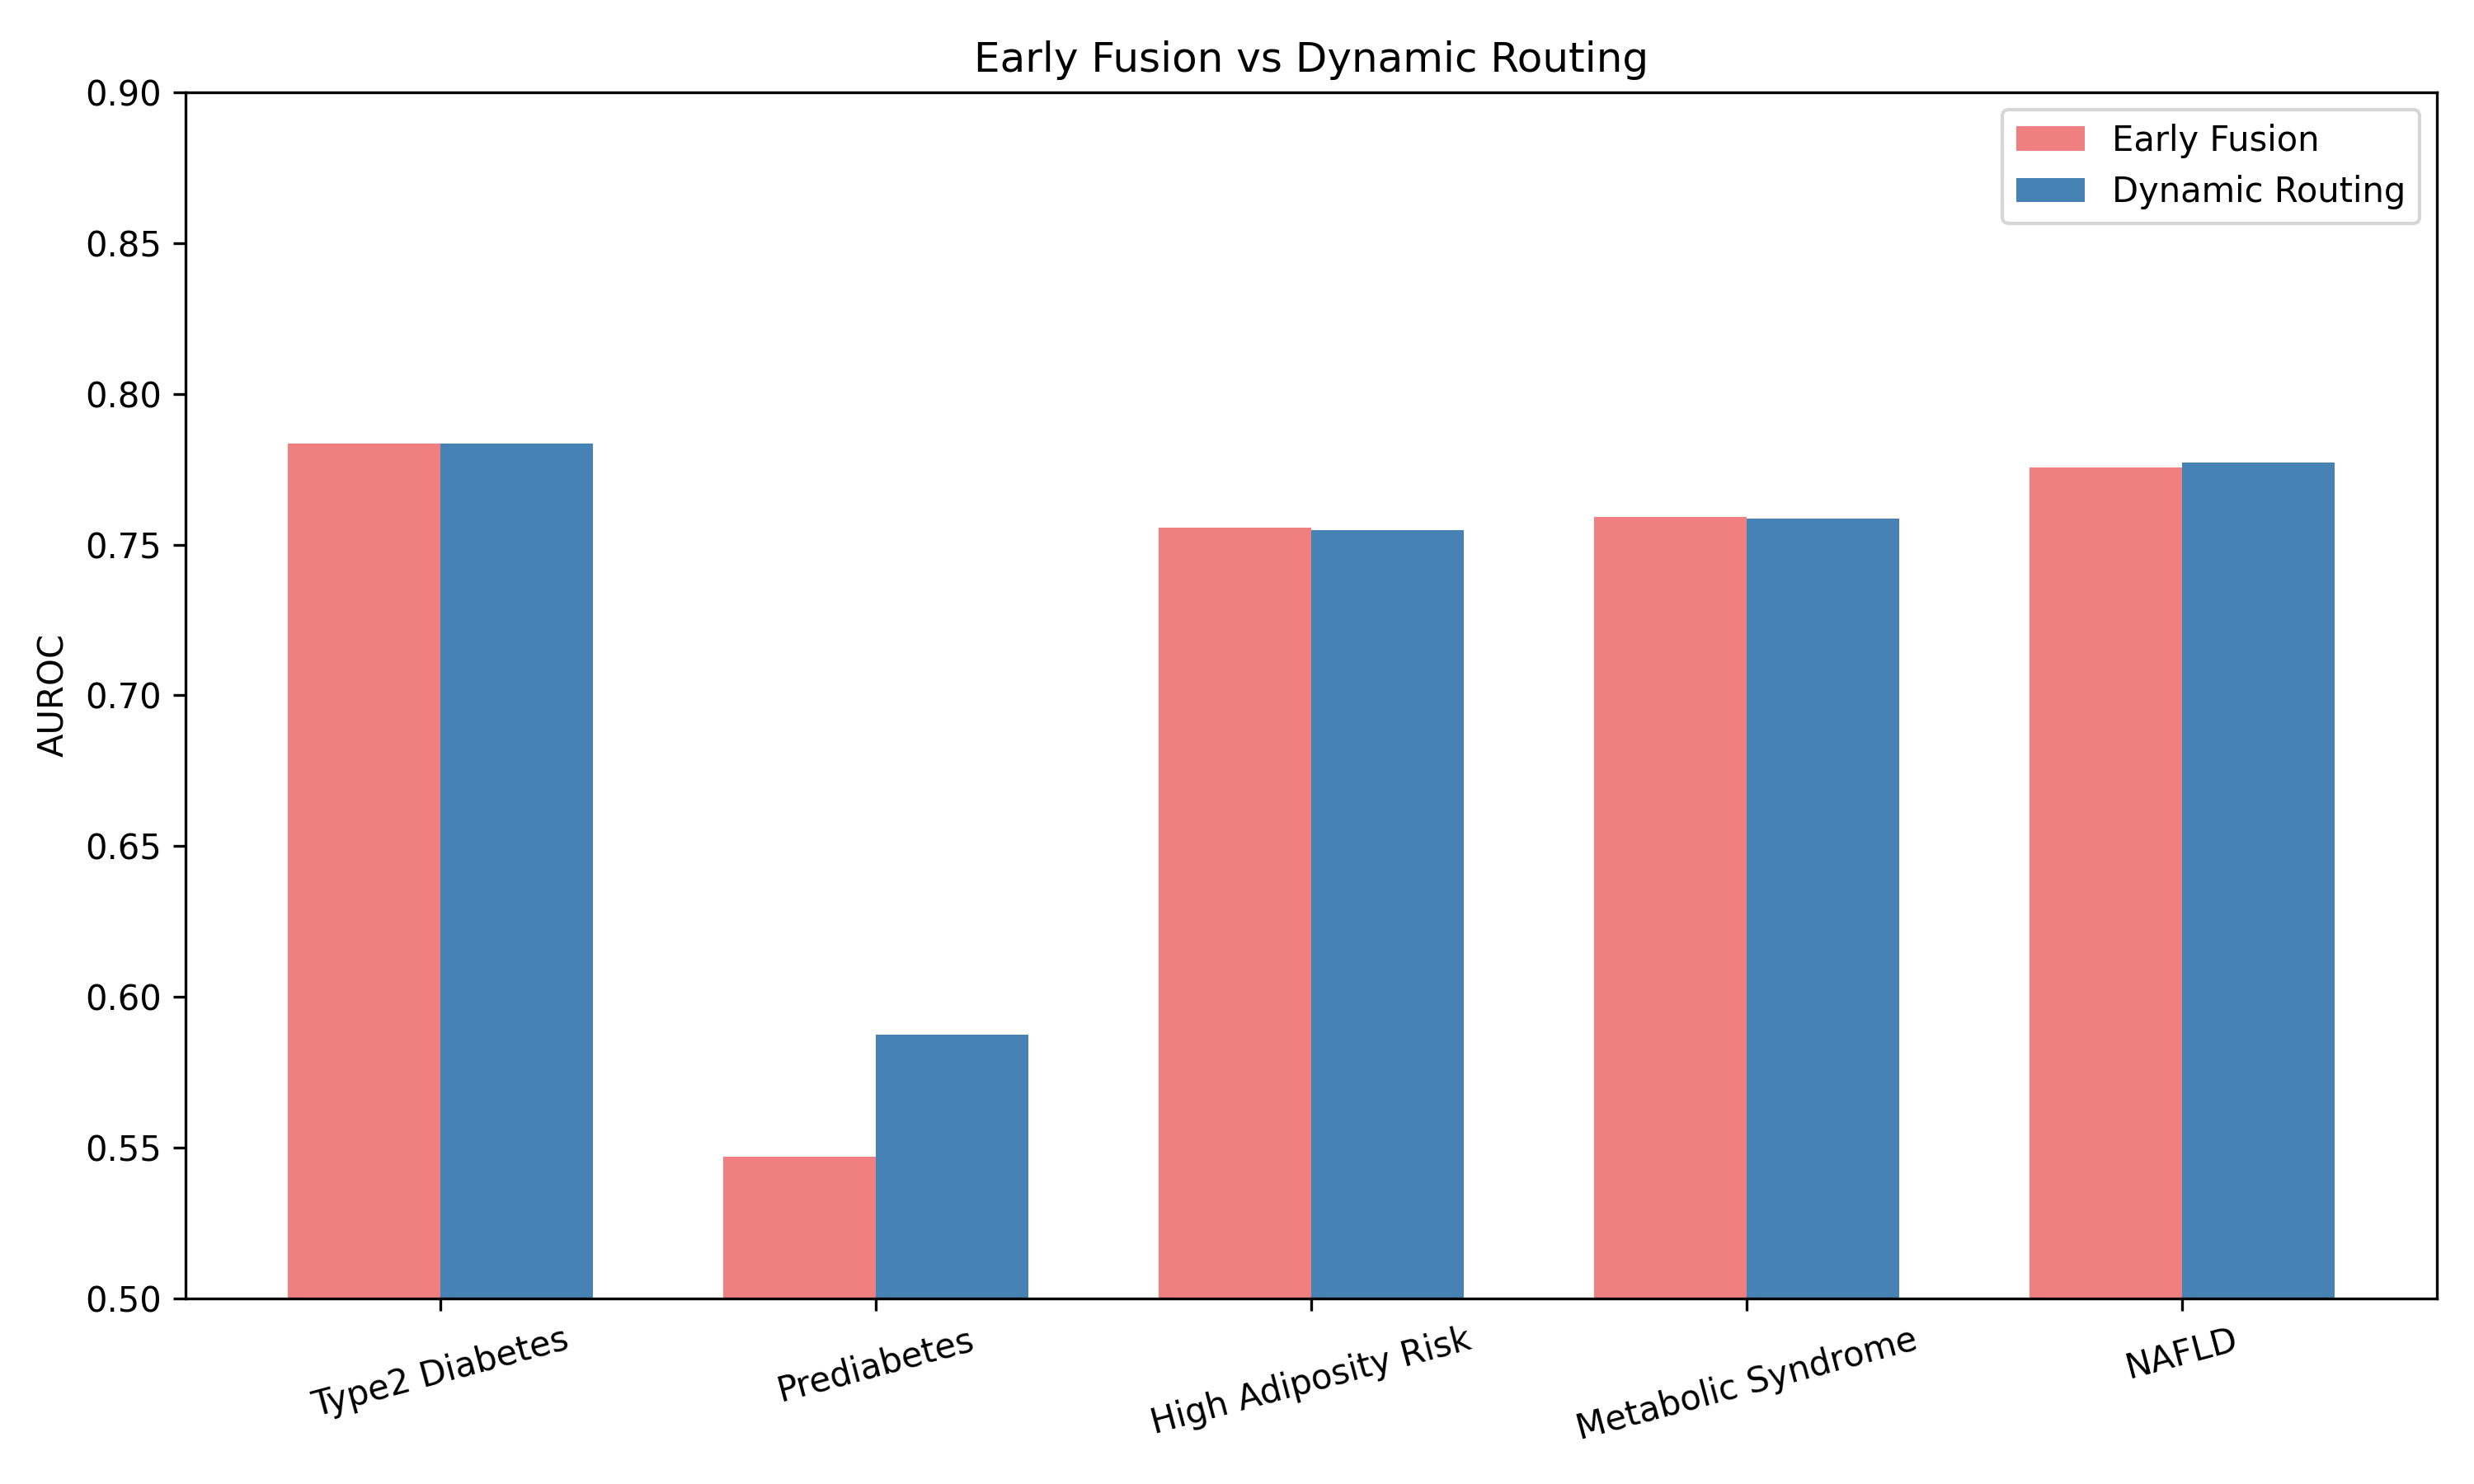
\includegraphics[width=\columnwidth]{figures/fig_early_vs_dynamic.png}
\caption{Side-by-side AUROC comparison of early feature-level fusion and dynamic probability-level routing for all five metabolic targets.}
\end{figure}

The two approaches performed within narrow margins for T2D (0.7836 vs.\ 0.7834), High Adiposity Risk (0.7557 vs.\ 0.7547), and Metabolic Syndrome (0.7591 vs.\ 0.7586). Dynamic routing surpassed early fusion for Prediabetes by 0.0405 (0.5875 vs.\ 0.5470) and for NAFLD by 0.0016 (0.7772 vs.\ 0.7756). Crucially, the early-fusion model is structurally rigid---it requires all 82 features to be present---whereas the routing architecture seamlessly accommodates any combination of available modalities.

\subsection{Explainability Outcomes}
Addressing RQ7, TreeSHAP attributions extracted from the tree-based experts consistently identified Fasting Glucose and HbA1c as the dominant clinical drivers for T2D risk, while BMI and Waist Circumference dominated the High Adiposity Risk pathway. Within the gut microbiome expert, Bacteroidetes relative abundance and Shannon Diversity emerged as leading contributors for several targets. These per-prediction attributions are passed to the Medical RAG module, which retrieves matching clinical guideline passages and composes narrative summaries that contextualize the quantitative risk scores within established medical knowledge.

\section{DISCUSSION}

\subsection{Primacy of Clinical Biomarkers}
The consistent superiority of the Clinical modality across all five targets aligns with established understanding that laboratory biomarkers---fasting glucose, HbA1c, lipid panels, and hepatic enzymes---carry dense metabolic information \citep{rajkomar2018scalable}. Within the context of this synthetic cohort, the clinical feature block was engineered to encode strong physiological correlates of each target, which the expert classifiers exploited effectively. This finding should be interpreted as a property of the data-generation framework rather than as evidence that clinical data universally outperforms other modalities in real-world settings.

\subsection{Incremental Value of Wearable and Microbiome Data}
Adding Wearable/CGM and Gut Microbiome channels to the Clinical baseline produced modest but consistent AUROC improvements---for example, from 0.7777 (C) to 0.7834 (C+W+G) for T2D. The magnitude of these increments suggests that, within the evaluated synthetic cohort, the additional modalities contribute complementary but not dramatically novel predictive information when clinical data is already available. Conversely, the W+G pathway demonstrates that non-clinical channels retain actionable discrimination (T2D AUROC 0.6894) when laboratory results are absent, an operationally important capability for resource-limited telehealth deployments.

\subsection{Dynamic Routing Versus Imputation}
The routing mechanism's advantage over median imputation, while numerically small (0.0021 at 30\% missingness), is directionally consistent and intuitively grounded: median-filling an entire absent modality injects population-average values that are uninformative for individual risk differentiation, whereas routing simply omits the missing channel. The widening gap with increasing missingness rates suggests that the cost of imputation noise grows as more patients are affected. However, the narrow margins preclude strong claims of superiority, and evaluation under informative missingness patterns (MAR, MNAR) remains necessary before clinical deployment.

\subsection{Late Versus Early Fusion}
The near-parity between probability-level routing and early feature concatenation demonstrates that the modular architecture sacrifices negligible discrimination relative to a monolithic model. The notable exception is Prediabetes, where dynamic routing achieved a 0.0405 AUROC advantage. Because Prediabetes exhibits the lowest prevalence (20.0\%) and the weakest overall signal, the ability of individual experts to specialize on their modality's distinctive signal may confer an advantage over a single model diluted by 82 heterogeneous features. The decisive practical benefit, however, is architectural flexibility: late fusion naturally accommodates missing modalities, whereas early fusion does not.

\subsection{Clinical Decision Support Considerations}
TeleMed-M3 illustrates how modality-aware routing, per-feature explanations via TreeSHAP, and RAG-grounded narrative generation can be composed into a cohesive telehealth decision-support pipeline. The routing layer ensures that patients are never excluded from risk assessment due to incomplete data, TreeSHAP furnishes actionable feature-level insights for clinician review, and the RAG module grounds the outputs in authoritative medical literature. Taken together, these components advance the framework beyond a black-box classifier toward a transparent, adaptable, and evidence-informed clinical tool---though clinical utility, workflow integration, and patient outcomes remain to be validated prospectively.

\section{LIMITATIONS}
Several constraints bound the generalizability of the reported findings:

\begin{enumerate}
    \item \textbf{Synthetic data only.} All experiments were conducted on a computationally generated cohort. The Gaussian Copula model \citep{xu2015sdv} captures pairwise linear dependencies but may fail to reproduce higher-order nonlinear interactions, rare phenotypes, and measurement artifacts characteristic of real patient data. No external validation on human cohorts was performed.
    \item \textbf{MCAR missingness assumption.} Modality absence was simulated via independent uniform removal, a strict MCAR mechanism. Clinical missingness is frequently informative---patients lacking microbiome data may systematically differ from those who have it---and performance under MAR or MNAR conditions is unknown.
    \item \textbf{Limited imputation baselines.} Only global median imputation was compared. More sophisticated approaches---multiple imputation by chained equations (MICE), $k$-nearest-neighbor imputation, variational autoencoders, and cross-modal generative models---were not benchmarked.
    \item \textbf{Fixed classification threshold.} F1 scores are reported at a fixed threshold of 0.5. Threshold optimization on a held-out calibration set and comprehensive calibration analyses (e.g., reliability diagrams, Hosmer--Lemeshow tests) were not performed.
    \item \textbf{Unvalidated RAG module.} The Medical RAG component is exploratory. Retrieval precision, generation faithfulness, hallucination rates, and clinician agreement were not quantitatively assessed.
    \item \textbf{Candidate algorithm scope.} The expert selection pool was limited to five classical and ensemble methods. Deep tabular architectures (e.g., TabNet, FT-Transformer) and neural stacking variants were not evaluated.
\end{enumerate}

\section{SAFETY AND CLINICAL POSITIONING}
TeleMed-M3 is expressly designed as a research-stage clinical decision-support framework and must not be misconstrued as an autonomous diagnostic or therapeutic system. The predicted risk probabilities and generated narrative summaries serve as supplementary information for qualified healthcare professionals; they are not substitutes for professional clinical judgment, laboratory confirmation, or guideline-directed patient management.

No claims of clinical efficacy, diagnostic accuracy on real populations, or treatment effectiveness are made. Before any patient-facing deployment, the system would require: (i) validation on appropriately consented, diverse human cohorts; (ii) calibration assessment under real-world prevalence and missingness distributions; (iii) evaluation against informative missingness mechanisms; (iv) usability testing with practicing clinicians; and (v) continuous post-deployment monitoring and human oversight.

\section{CONCLUSION}
This paper introduced TeleMed-M3, a probability-level multimodal learning framework that unifies Clinical, Wearable/CGM, and Gut Microbiome data streams for five-target metabolic risk stratification within a telemedicine architecture. By decoupling modality-specific expert training from cross-modal fusion, the system routes each patient through the appropriate subset of seven non-empty modality-availability pathways, eliminating the need to synthetically reconstruct any wholly absent data channel.

Evaluation on a controlled 100{,}000-patient synthetic cohort demonstrated that clinical biomarkers constitute the dominant predictive signal, while supplementary wearable and microbiome channels yield consistent---though modest---improvements in discrimination. Under simulated MCAR conditions, dynamic routing maintained higher AUROC than median imputation across all tested missingness rates, and probability-level stacking matched or exceeded early feature-level fusion on every target. TreeSHAP attributions provided transparent, per-feature explanations for individual risk assessments, and an exploratory Medical RAG layer illustrated the feasibility of grounding model outputs in authoritative clinical guidelines.

Looking ahead, validation on real-world multimodal clinical datasets, evaluation under informative missingness patterns, benchmarking against advanced imputation and deep fusion methods, and prospective clinical studies are essential steps toward translating this research framework into a deployable telehealth tool. Quantitative evaluation of the RAG module's generation quality and clinician acceptance testing represent additional high-priority directions.

\section*{Reproducibility and Data Availability}
The complete codebase---encompassing synthetic data generation scripts, model training pipelines, fusion and routing logic, evaluation notebooks, and reproducibility audit logs---is available in the project repository. Because the dataset is entirely synthetic, it can be regenerated from the provided configuration parameters without implicating patient privacy. All random seeds, hyperparameter configurations, and train/validation/test split indices are recorded to enable exact replication of the reported results.

\bibliographystyle{apalike}
\bibliography{references}

\end{document}
